
\chapter{Background} \label{sect-background}
In this chapter we introduce the tools which we have evaluated namely \emph{LIME}, \emph{SHAP}, and \emph{Lucid}. We also explain in detail how these tools provide explanations.
\section{LIME}
\textbf{LIME} \emph{(Local Interpretable Model-Agnostic Explanations)} \cite{lime} is a model-agnostic explainer which attempts to provide an interpretable \emph{explanation model} for any supervised learning problem. The overall idea of LIME is to provide an explanation for a complex model by approximating it locally with an \emph{interpretable} one which is referred to as the \emph{explanation model}. It is considered a \emph{local} interpretation as LIME can only explain a single prediction at a time. This is done by choosing a single instance and transforming it into a representation that LIME can understand which is explained in Section \ref{sect-Internal}. Small perturbations of the transformed instance is generated which are close in proximity to the instance. The way these perturbations are generated is dependent on the type of the input and the methods include adding noise to continuous features, removing words or hiding parts of an image.  This is discussed further in Section \ref{sect:sampling-lime}. The perturbed samples are then predicted by the original model. The interpretable model is trained by using the perturbed samples as the input and their corresponding predictions from the original model as their labels which is explained in detail in Section \ref{sect:lime-expl-train}. The weights from the explanation model are extracted and are considered a local explanation for the chosen instance as we are able to monitor how the change in specific features brought upon by the perturbations affect the outcome of the prediction. The explanation model is represented by the following linear equation,
\begin{equation}
g(z^{'}) = \phi_0 + \sum\limits_{i=1}^M \phi_i z_{i}^{'}
\label{eq:lime-explanation}
\end{equation}
where $z^{'} \epsilon$ $\{0,1\}^{M}$ represents a simplified input which is explained in chapter \ref{sect-Internal}, M is the number of simplified input features, and $\phi_{i}$ $\epsilon$ $\mathbb{R}$ is an attribute value assigned to each feature indicating their impact on the prediction \cite{NIPS2017_7062}.
The \emph{explanation model} is used as an approximation for the complex model and remains linear so that it is interpretable. We can see from (\ref{eq:lime-explanation}) that we only have a relationship between our inputs $z^{'}$ and prediction $g(z^{'})$. This means that the explanation is rather limited as we are unable to gather any information regarding the hidden layers. Suppose we have a model which takes in a list of symptoms that a patient is exhibiting and attempts to predict whether the patient has the flu or not, in figure \ref{fig:lime-process} we can see how LIME takes the input features which are the symptoms of the patient and provides visual feedback where each feature is given a weight which is represented by the length of the bar of the feature and a color representing how much they contributed towards or against the patient having the flu. Ultimately the visual feedback is given to a Doctor as a reference and they should be the one to give the final diagnosis.




\begin  {figure} [!htbp]
  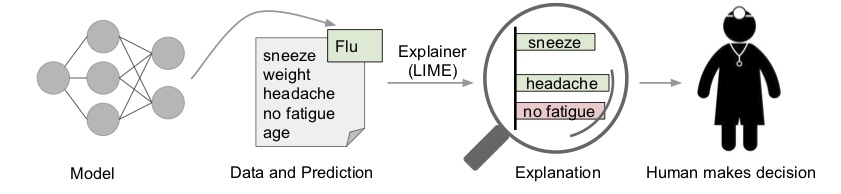
\includegraphics[width=\linewidth]{Evaluation_Images/Lime_Process.jpg}
  \caption{Example of LIME on a model that predicts whether a patient has the flu. \cite{lime}}
  \label{fig:lime-process}
\end{figure}


\subsection{Internal data representation} \label{sect-Internal} Before the model can be explained, LIME performs a transformation on the input to create it's own internal representation that it can interpret. The transformation is done behind the scenes and is dependent on the type of the input data.

\begin{itemize}
\item For text data a model would commonly use complex representations such as word embeddings but a simpler representation is needed such as a binary vector where 1 indicates the presence and 0 the absence of a given word. This can be formally expressed as, 
$X^{'}={\{0,1\}}^{p}$ where $p$ is the number of words in the instance being explained. For example given a corpus of words \{The, cat, dog, jumped, leaped, over, under, the, fence\} and the input sentence  ``The dog jumped over the fence'', we could represent the input with the binary vector \{1, 0, 1, 1, 0, 1, 0, 1, 1\}.

\item For images a binary vector is used to indicate the presence or absence of super pixels \cite{10.5555/946247.946677} which is a grouping of similar pixels in the image, where 1 indicates that the original value of the super pixel is used and 0 the pixel is set to grey which represents missing. This can be formally expressed as, $X^{'} = {\{0,1\}}$ where $p$ is the number of identified super pixels in the input image. Identifying super pixels is usually done by image segmentation algorithms such as Quickshift \cite{10.1007/978-3-540-88693-8_52}.

\item For tabular data such as matrices it is dependent on the type of data. In the case of numerical data the representation is simple enough so the identity mapping is used $X^{'} = X$. For categorical data a binary vector is once again used which can be formally expressed as $X^{'}={\{0,1\}^{p}}$ where $p$ is the number of features used by the model. In the binary vector 1 indicates that the feature takes on the original category and 0 indicates that the feature is mapped to a different category sampled according to the distribution of the training data. Categorical data, is data which is grouped into some sort of category or multiple categories. For example, a categorical feature would be used to represent the type of an animal which could be either a cat, dog, or mouse. In this case we would have 3 categories and we could use a 0 to present the category cat, 1 to represent the category dog, and 2 to represent the category mouse.
\end{itemize}
Regardless of the data type, LIME creates a mapping function which transforms the internal data representation back into its original form for use when predicting on the actual model.

\subsection{Sampling from the input} \label{sect:sampling-lime} Once the the input has been transformed into a internal representation, LIME begins sampling from the new input in order to create perturbed samples. The sampling process like the data transformation process is dependent on the type of input data.

\begin{itemize}
\item For text data, the sampling process involves removing uniformly at random, words from the instance. In the previous example ``The dog jumped over the fence'', some permutations that could be created from sampling would be ``dog jumped over the fence'', ``over the fence'', or ``jumped''.

\item For images, the sampling process is as simple as setting  values chosen uniformly at random in the vector to 0 therefore setting them to missing.

\item For tabular data such as matrices, it is once again dependant on whether the data is numerical or categorical. For categorical features we randomly set features to 0 so that they take random values within their category. For numerical features, the instance is perturbed by sampling from a normal distribution and doing the inverse operation of mean-centering and scaling.
\end{itemize}



\subsection{Training the explanation model} \label{sect:lime-expl-train} Finally the explanation model has to be trained, given a prediction instance $x$, i.e. a specific feature set that predicts a specific probability under the model, after LIME has transformed the input into a internal data representation $x^{'}$ and a specified number perturbed samples have been generated. An individual perturbed sample $z$ is then reconstructed to represent an actual sample if needed. This is mainly done by setting the missing features to 0. The reconstructed input $z^{'}$ is predicted on the model and LIME records how the new prediction probabilities have changed. This is done for each perturbed sample, the more perturbed samples we use the more accurate the results are. By doing this LIME is able to explain the contribution of each feature towards the prediction.
We choose the \emph{explanation model} by using the following equation,
\begin{equation}
\xi(x) = \argmin_{g\epsilon G} L (f, g,\pi_{x} ) + \Omega(g)
\label{eq:explanation-loss}
\end{equation}
where f is the model that we are trying to explain, g is all potential explanation models, $\xi(x)$ represents the optimal explanation model, $L(f, g, \pi_{x})$ is the approximation of the difference between f and g, $\pi_{x}$ is a proximity measure between an instance z to x to define locality around x where instances closer to x are given a higher weighting, and $\Omega(g)$ is a complexity score given to the current explanation model which needs to minimized . LIME defaults to linear sparse models which are given a complexity rating $\Omega(g) = 0$  as the domain for possible explanation models such as in (\ref{eq:lime-explanation}).
We can see in figure \ref{fig:lime-boundary} the linear decision boundary that LIME has learnt within a complex space. The crosses represent the perturbed sampled which were generated training the explanation model, where the bold cross is the initial input. The complex space is the models decision function and the dotted line is the linear explanation model that LIME has learnt.

\begin  {figure}[!htpb]
\centering
  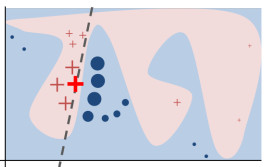
\includegraphics[width=0.7\linewidth]{Evaluation_Images/Lime_boundary.jpg}
  \caption{Linear decision function learnt in complex space \cite{lime}.}
  \label{fig:lime-boundary}
\end{figure}



\subsection{Providing feedback to the user}
The end goal of LIME is to provide textual and visual artifacts to the end user that explains the chosen prediction. The \emph{explanation model} itself is used as the explanation for the chosen prediction. The feature attributes $\phi_{i}$ are presented to the user in a representation that is interpretable by humans.
\begin{itemize}
\item For  feedback on a image-based model, suppose we had a model which attempts to predict whether a given image is of an \emph{Electric guitar}, \emph{Acoustic guitar}, or \emph{Labrador}. In figure \ref{fig:lime-visual-feedback}, for the 3 respective classes the relevant super pixels which had a positive impact on the prediction of that particular class are displayed and the rest of the image is greyed out.
\item In the case of a model trained on text data, suppose we had a model which given an article attempts to predict whether the topic is about \emph{Atheism} or \emph{Christianity}. In figure \ref{fig:lime-textual-feedback} we can see the prediction probabilities of each class and the words which attributed towards the prediction are highlighted and given a weighting.
\end{itemize}

\begin  {figure}[!htpb]
  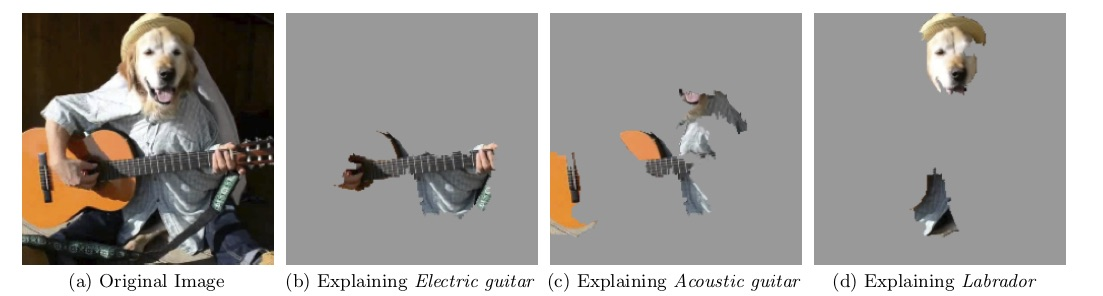
\includegraphics[width=\linewidth]{Evaluation_Images/Lime_visual_representation.jpg}
  \caption{Example of visual feedback \cite{lime}. }
  \label{fig:lime-visual-feedback}
\end{figure}

\begin  {figure}[!htpb]
  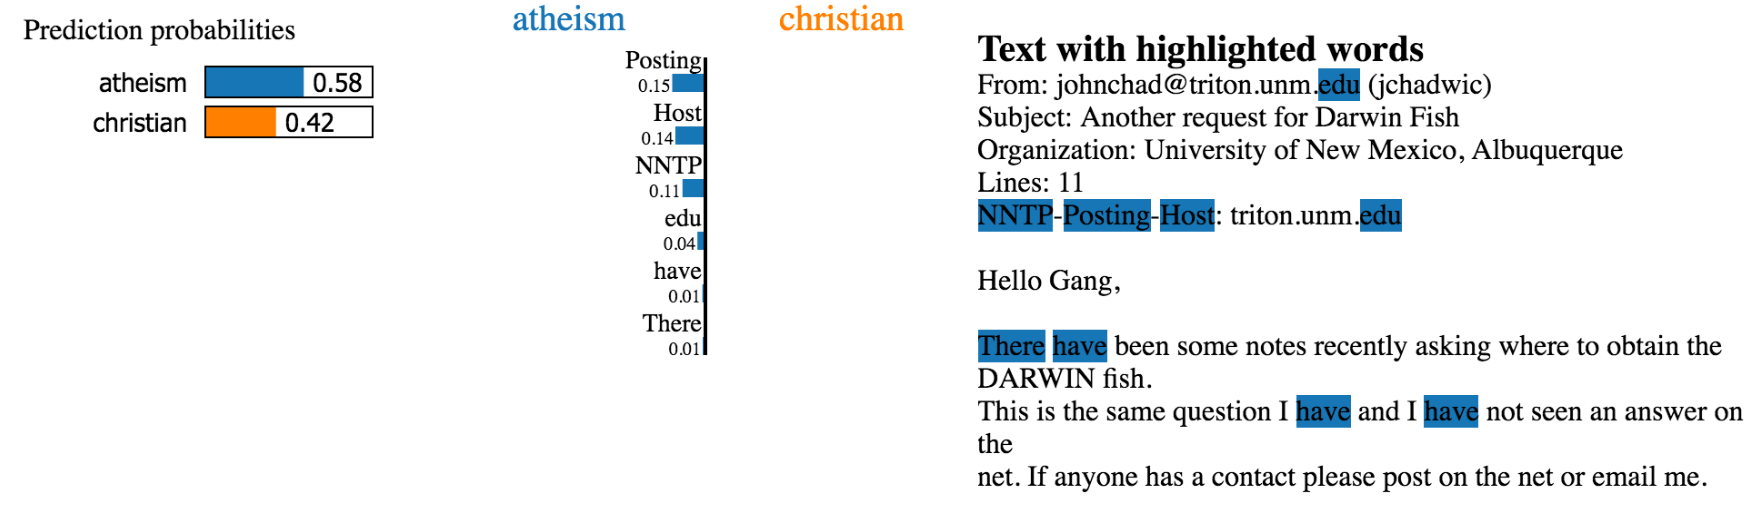
\includegraphics[width=\linewidth]{Evaluation_Images/Lime_text_represntation.png}
  \caption{Example of textual feedback \cite{Https://github.com/marcotcr/lime}.}
  \label{fig:lime-textual-feedback}
\end{figure}

\subsection{SP-LIME}
Since LIME is only able to provide an explanation for a single prediction at a time, it is up to the user to explain multiple instances in order to gain a global understanding of the model. A tool called Submodular Pick LIME (SP-LIME) \cite{lime} is used to help the user choose instances that do not overlap and each extra instance should bring a better understanding of the model on a global level. A human is only willing to view a certain number of explanations in order to understand a model and this is denoted as $B$ instances. A \emph{pick step} is provided which selects  the optimal $B$ instances for the user to inspect. The pick step aims to pick a diverse set of explanations that are non-redundant to show the user in order to explain how the model behaves globally. We denote $W$ as being an \emph{explanation} matrix that represents the local importance of the interpretable components for a set of instances $X (|X| = n)$ \cite{lime}. Each row in $W$ denoted as $i$ represents an instance and each column denoted as $j$ represents each feature or component. We denote $I_{j}$ as the global importance of that component in the explanation space. Intuitively,  we  want $I$ such  that features that explain many different instances have higher importance scores. An example of how the pick algorithm operates can be seen in Figure \ref{fig:sp-lime-example}. The rows represent instances and the columns are features. The goal is to choose new instances so that new features are being explored. If the second row was one of the picked explanations then there would be no reason to chose the third row as they both explain the same set of features $f2$ and $f3$. The fifth row would be a good instance to pick as it explains a distinct set of features $f4$ and $f5$. Using our importance function $I$ it should score feature $f2$ higher than feature $f1$, i.e. $I_{2} > I_{1}$ since $f2$ is used to explain more instances. This non-redundant  coverage intuition can be formally expressed as,
\begin{equation}
    c(V,W,I) = \sum^{d'}_{j=1} \mathds{1}_{[\exists i \epsilon V : W_{ij} > 0]}I_{j}
    \label{eq:coverage-inution}
\end{equation}
where we define coverage as the set function c that, given W and I, computes the total importance of the features that appear in at least one instance in a set V.
The pick problem can be defined as,
\begin{equation}
   \mbox{Pick}(W,I) = \argmax_{V,|V|\leq B} c(V,W,I)
\end{equation}
consists of finding the set $V ,|V| \leq B$ that achieves highest coverage. This is algorithm is known as \emph{submodular pick} and is a NP-hard problem \cite{10.1145/285055.285059}.
\begin  {figure}[!htpb]
\centering
  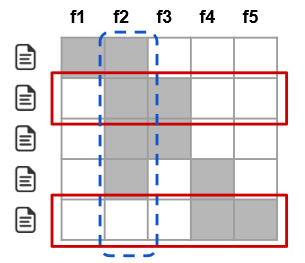
\includegraphics[width=0.5\linewidth]{Evaluation_Images/SP-LIME-Example.png}
  \caption{Toy  example $W$. Rows  represent  instances (documents) and columns represent features(words).  Feature f2 (dotted blue) has the highest importance.  Rows 2 and 5 (in red) would be selected by the pick procedure, covering all but feature f1 \cite{lime}.}
  \label{fig:sp-lime-example}
\end{figure}


\subsection{Limitations} LIME works as well as the explanation model that is built, if the explanation model does not approximate the real model well then LIME will not perform well in turn. Since LIME attempts to provide visual and textual artifacts to the user for interpretation, if there are many features such as in the thousands then even if the interpretation is accurate, a human will not be able to interpret so much information. LIME is also only able to interpret a single prediction at a time, this may not be representative of how the model performs on a global scale so it is up to the user to properly make use of this in order to gain global understanding of their model.


\section{SHAP}

SHAP(Shapley Additive exPlanations) \cite{NIPS2017_7062} is a tool which combines and adapts various different interpretation tools with LIME being one of them. It can be shown that these different tools all attempt to create the same explanation model in the form of (\ref{eq:lime-explanation}) and are referred to as \emph{additive feature attribution methods} \cite{NIPS2017_7062}. These tools were all created in isolation and there was no simple way to determine when one method was preferable to another.  It can be shown that there is a single unique and desirable solution between these different  \emph{additive feature attribution methods} that adheres to three desirable properties derived from Shapley value estimation methods \cite{articleb} \cite{article} \cite{inproceedings}. These properties are \emph{local accuracy}, \emph{missingness}, and \emph{consistency} which we will further discuss in chapter \ref{sect:shap-properties}. From this unique solution, \emph{SHAP values} \cite{NIPS2017_7062} are derived which can be seen as a unified measure of feature importance.
\subsection{Properties} \label{sect:shap-properties}

\subsubsection{Local Accuracy}
Requires the \emph{explanation model} $g$ to at least match the output of the original model $f$ for the simplified input $x^{'}$ (which corresponds to the original input x),
\begin{equation}
    f(x) = g(x^{'}) = \phi_{0} + \sum\limits_{i=1}^M \phi_i x_{i}^{'}
    \label{eq:accuracy}
\end{equation}
where $M$ is the number of simplified inputs and $\phi_{i}$ are their values.


\subsubsection{Missingness}
Constrains features where $x^{'}_{i}= 0$ to have no attributed impact. 

\begin{equation}
x^{'}_{i} = 0 \Longrightarrow \phi_{i} = 0
\label{eq:missingness}
\end{equation}


\subsubsection{Consistency}
 If a model changes so that some simplified input’s contribution increases or stays the same regardless of the other inputs, that input’s attribution should not decrease. Let $h_x(x^{'})$ be a mapping function that transforms a simplified input $x^{'}$ into the original input $x$, $f_{x}(z^{'}) = f(h_{x}(z^{'}))$ and $z^{'} \setminus i$ denote setting $z_{i}^{'} = 0$. For any two models $f$ and $f^{'}$, if
 \begin{equation}
    f^{'}_{x}(z^{'}) - f^{'}_{x}(z^{'} \setminus i) \geq f_{x}(z^{'}) -  f_{x}(z^{'} \setminus i)
    \label{eq:consistency}
 \end{equation}
 for all inputs $z^{'} \epsilon\{0, 1\}^{M}$, then $\phi_{i}(f^{'}, x) \geq \phi_{i}(f, x)$.
 
 \subsection{Unique solution}
 
SHAP then introduces a single unique solution which can be written as an  \emph{Additive feature attribution method} and adheres to all 3 three properties.

\begin{equation}
    \phi_{i}(f, x) = \sum\limits_{z^{'} \subseteq x^{'}} \frac{|z^{'}|!(M - |z^{'}| - 1)!}{M!}[f_{x}(z^{'}) - f_{x}(z^{'} \setminus i)]    
    \label{eq:unique}
\end{equation}
where $|z^{'}|$ is the number of non-zero entries in $z^{'}$, and $z^{'} \subseteq x^{'}$ represents all $z^{'}$ vectors where the non-zero entries are a subset of the non-zero entries found in $x^{'}$.
This equation was derived from cooperative game theory results, where the values $\phi_{i}$ are referred to as Shapley values \cite{Shapley1952value}. It has been proven that Shapley values adhere to properties 1 and 3, but not 2. The previous \emph{additive feature attribution methods} such as LIME are proven to sometimes violate properties 1 and 3, but adhere to property 2. Thus the previous \emph{additive feature attribution methods} are adapted to use Shapley values so that they adhere to all 3 properties and therefore is the solution to (\ref{eq:unique}). We discuss how these techniques are adapted to use Shapley values in chapter \ref{sect:shap-explainers}. A new unified measure of feature importance is proposed called \emph{SHAP Values}  \cite{NIPS2017_7062} which is the solution to (\ref{eq:unique}) and is used to adapt previous \emph{attribution methods}

\subsection{SHAP Values}
\emph{SHAP Values} are the Shapley values of a conditional expectation function of the original model, which means they are the solution to (\ref{eq:unique}), where $f_{x}(z^{'}) = f(h_{x}(z^{'}))) = E[f(z) | z_{S}]$, and S is the set of non-zero indexes in $z^{'}$ \cite{NIPS2017_7062}. Although the exact computation of SHAP values are challenging, by combining insights gathered from current \emph{additive feature attribution methods} it is possible to approximate them.
SHAP makes two other assumptions  \emph{model linearity} and \emph{feature Independence} in order to further simply the expected values,
\begin{equation*}
f(h_{x}(z^{'})) = E[f(z) | z_{S}],
\end{equation*}
\text{ applying our two assumptions we can simplify this as,}
\begin{equation}
\approx f([z_{S}, E[z_{\overline{S}}]])
\label{eq:summarized-unique}
\end{equation}
SHAP (Shapley Additive exPlanation) values attribute to each feature the change in the expected model prediction when conditioning on that feature.  They explain how to get from the base value $E[f(z)]$ that would be predicted if we did not know any features to the current output $f(x)$ \cite{NIPS2017_7062}. Figure \ref{fig:shap-values} shows a single ordering. In the case of features which are dependant on one another or a nonlinear model, the order of which the features are added to the expectation is important.  In that case the SHAP values are calculated by averaging the $\phi_{i}$ values across all possible orderings \cite{NIPS2017_7062}. 
\begin  {figure} [!htbp]
  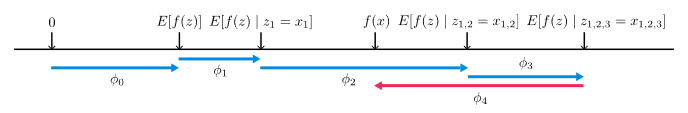
\includegraphics[width=\linewidth]{Evaluation_Images/Shap_values.png}
  \caption{How the SHAP values are computed. \cite{NIPS2017_7062}}
  \label{fig:shap-values}
\end{figure}

\subsection{Types of explainers} \label{sect:shap-explainers}
Using SHAP Values, the previous \emph{additive feature attribution methods} can be adapted. There are a total of 6 tools which are adapted, however in this paper we only look at the adaptions of LIME and DeepLIFT\cite{DBLP:journals/corr/ShrikumarGK17}\cite{DBLP:journals/corr/ShrikumarGSK16}.

\subsubsection{Kernel SHAP}
Adapting LIME to adhere to properties 1 and 3 which it initially violates gives rise to \emph{Kernel SHAP}, which makes use of SHAP Values. It remains model agnostic. If we refer back to (\ref{eq:explanation-loss}), we recall that $\Omega(g)$ is the term which penalizes the \emph{explanation model} based on how complex it is, $\pi_{x^{'}}$ is the locality around input $x^{'}$, and $L(f, g, \pi_{x^{'}})$ is the loss function which indicates the difference between the original model $f$ and the explanation model $g$. These three values are determined heuristically by LIME. However SHAP \cite{NIPS2017_7062} provides methods for choosing them that adheres to all three properties and has been named \emph{Shapley Kernel}.
Under (\ref{eq:lime-explanation}), the specific forms of $\pi_{x^{'}}$, L, and $\Omega$ which make (\ref{eq:explanation-loss}) consistent with the three properties of SHAP are:
\begin{align*}
   \Omega(g) = 0,
\end{align*}
\begin{align*}
    \pi_{x^{'}}(z^{'}) = \frac{(M-1)}{{M \choose |z^{'}|}|z^{'}|(M-|z^{'}|)},
\end{align*}
\begin{align*}
    L(f,g,\pi_{x^{'}}) = \sum\limits_{z^{'}\epsilon Z} [f(h_{x}(z^{'})) - g(z^{'})]^{2} \pi_{x^{'}}(z^{'}),
\end{align*}
where $|z^{'}|$ is the number of non-zero elements in $z^{'}$. $\Omega(g)$ remains 0 because we still use linear models, $\pi_{x^{'}}(z^{'})$ is the weighting of how close the sampled input $z^{'}$ is to the simplified input $x^{'}$  where $M$ is the number of features in $x^{'}$, and $L(f,g,\pi_{x^{'}})$ is the mean squared error which depends on the weighting of $\pi_{x^{'}}(z^{'})$. 


\subsubsection{Deep SHAP}
DeepLIFT was proposed as a recursive prediction explanation model for deep learning \cite{DBLP:journals/corr/ShrikumarGSK16}\cite{DBLP:journals/corr/ShrikumarGK17}. The user assigns each feature a reference value which is typically a background feature for that particular feature. For each input $x_{i}$ a value $C_{\Delta{x_{i}}\Delta{y}}$ is given which represents the effect of setting that particular input to it's reference value. Once again we introduce the mapping function $x = h_{x}(x^{'})$ that converts a simplified binary input $x^{'}$ to the original input $x$, where 1 indicates the input takes it's original value and 0 it takes it's reference value.
DeepLIFT therefore uses the following property named the ``summation-to-delta property'' \cite{NIPS2017_7062},
\begin{equation}
    \sum\limits_{i=1}^{n}C_{\Delta{x_{i}}\Delta{o}} = \Delta{o},
    \label{eq:deeplift}
\end{equation}
    where $o = f(x)$, $\Delta{o} = f(x) - f(r)$, $\Delta{x_{i}} = x_{i} - x_{r_{i}}$, and $r$ is the reference input.
    (\ref{eq:deeplift}) can be written in the form of (\ref{eq:lime-explanation}) by setting $\phi_{i} = C_{\Delta{x_{i}}\Delta{o}}$ and $\phi_{0} = f(r)$, therefore it is an \emph{additive feature attribution method}.
Although \emph{Kernel SHAP} is completely model-agnostic, we can leverage extra knowledge abut deep networks in order to increase computational performance. DeepLIFT on it's own only satisfies the local accuracy and missingness properties, but if we interpret the reference values $r_{i}$ as $E[x]$ in  (\ref{eq:summarized-unique}) then DeepLIFT approximates SHAP values and consistency is also adhered to given that the model is linear and the features are independent of one another. The new method is labeled \emph{Deep SHAP} which not only computes SHAP Values but also combines the values computed for smaller components of the network into values for the whole network \cite{NIPS2017_7062}.


\subsection{Limitations}
SHAP has a similar limitation to LIME as that it only uses the input and output of a model for interpretation and therefore no knowledge of hidden layers is achieved. SHAP also assumes \emph{model linearity} and \emph{feature independence} which is an assumption which more complex models may not adhere to. SHAP is also more computationally intensive than LIME due to extra constraints and the need to approximate Shapley values.




\section{Lucid}
Lucid is a collection of infrastructure and tools for research in neural network interpretability \cite{Https://github.com/tensorflow/lucid}. Several powerful techniques such as \emph{feature visualization}, \emph{attribution}, and \emph{dimensionality reduction} have been studied for interpreting neural networks, however these techniques have been researched in isolation and there has been not been research on how these techniques may complement one another. Lucid is primarily focused on interpretability into image-based networks such as CNNs where various parts of Lucid can be used in order to gain some interpretation into the hidden layers, the previously isolated interpretation techniques have been unified to create a rich interface \cite{olah2018the}. The interface that Lucid provides can be seen in figure \ref{fig:lucid-summary}, the \emph{layers} are the layers which we are able to gain insight into, \emph{atoms} are the various ways we can group the the pixels in the input images which will be explained further in chapter \ref{sect:lucid-activations}, \emph{content} is the type of information we can gain, and \emph{presentation} is how this information is relayed to the user \cite{olah2018the}. 

\begin  {figure}[!htpb]
  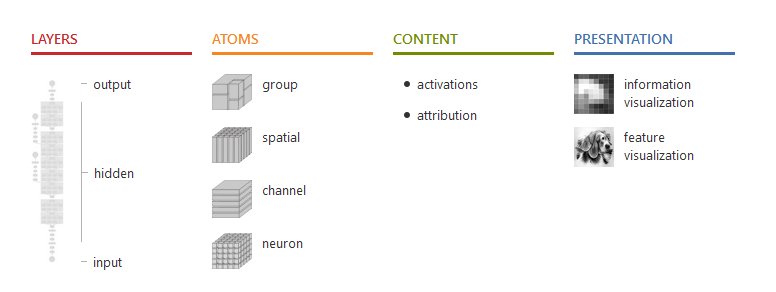
\includegraphics[width=\linewidth]{Evaluation_Images/LUCID_SUM.png}
  \caption{The interface that Lucid provides. \cite{olah2018the}}
  \label{fig:lucid-summary}
\end{figure}



\subsection{Semantic dictionaries}
The previous two tools \emph{LIME} and \emph{SHAP} only attempt to provide interpretation  between input and output layers, where as Lucid provides interpretation between any two layers. Each layer in a neural network can be seen as a three-dimensional cube where each cell represents an \emph{activation}, which is the amount that a specific neuron fires. The x- and y-axes represent the positions in the image, and the z-axes the particular channel. Usually activations are represented as abstract vectors that are not interpretable. A \emph{Semantic dictionary} is introduced which provides a more meaningful human interpretable representation of activations. \emph{Semantic Dictionaries} attempt to provide each activation with a \emph{canonical example} by mapping each activation with a visualization of that particular neuron sorted by the magnitude. This allows activations to map to similar human representations such as a ``Floppy ear'', or ``Dog snout'' when interpreting a model trained on classifying dogs. There are many ways to approximate the relationship between features and how they are used to arrive at a prediction however in this case they are linearly approximated.

\subsection{Types of Activations} \label{sect:lucid-activations} 
Since we can visualize the group of neurons as a cube, there are different ways we can slice this cube into groupings to form activations. The way each activation breaks up the cube can be seen in figure \ref{fig:lucid-maps}
.
\subsubsection{Individual Neurons}
A \emph{Saliency map} \cite{10.1023/A:1012460413855} is a simple heat map which highlights pixels of a input image that cause the most output classification. Since this method works with each individual neuron we run into two big problems, each pixel in a image is usually entangled with surrounding pixels and is heavily affected by transformations such as contrast or brightness changes. The second problem is that \emph{saliency maps} are fairly limited and do not allow multiple class attributions to be displayed at one time.

\subsubsection{Spatial Activations}
Due to the limitations of the previous approach only being able to show the attributions to a single class at a time, a different approach is introduced called \emph{Spatial activations} \cite{olah2018the}. Spatial activations are performed from a chosen layer to all $n$-output classes. Dimensionality reduction is then performed on this n-dimensional vector to produce a multi-directional \emph{saliency map}. Once this \emph{saliency map} is overlayed on the magnitude-sized activation grid we obtain an \emph{information scent} over this attribution space. This allows attribution between layers, however different concepts are being detected together and if we continue to use spatial positions these concepts will remain entangled.

\subsubsection{Channel Activations}
A \emph{channel} can be seen as a specific layer or view of an image. There are detectors at each channel representing a different view of the image. For a  normal color image we have the width and height to represent the pixels and the channels are the 3 color channels. In more complex representations of images these channels can be specialized to detect certain features such as eyes or noses.  By using spatial activations, the attribution is aggregated over all channels. which means we can not tell which detectors at each position most contributed to the final output classification. We can slice the cube by channels rather than spatial locations, which allows us to tell which detectors contributed the most to the output. In the case of a model which attempts to classify dogs, detectors may include those which detect ``Floppy ears'' or ``Dog snouts''.
\subsubsection{Neuron Groups}
\emph{Individual neurons} can provide the most information, however for larger networks where there may be tens of thousand of neurons this is too much information for humans. \emph{Spatial activations} and \emph{Channel activations} both provide different information about the layers, however we would gain the most if we could combine both of these techniques. There is a field of research, called \emph{matrix factorization} which studies optimal ways of breaking up matrices, we can make use of these methods by flattening the cube into a matrix of spatial locations and channels. Applying \emph{matrix factorization} on this newly created matrix, we can obtain more meaningful explanations of the layers.  By using the techniques in \emph{matrix factorization} we are able to choose what we prioritize in the activations such as describing the gradient, fully describing the activations, or if we want to fully describe the attributions. The problem with this method is that the \emph{neuron groupings} we use for a particular image can not be used for another image as each image would require a unique set of groups. 
\begin  {figure}[!htpb]
  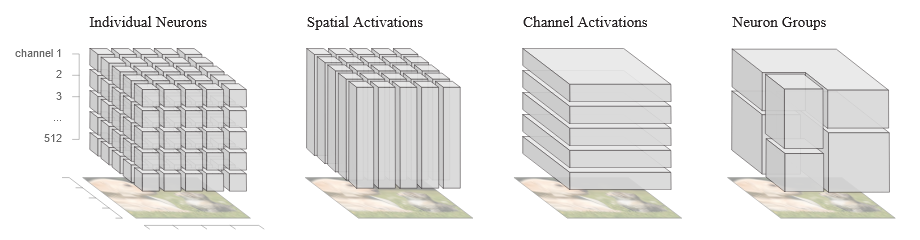
\includegraphics[width=\linewidth]{Evaluation_Images/LUCID_maps.png}
  \caption{Different types of activations. \cite{olah2018the}}
  \label{fig:lucid-maps}
\end{figure}




\subsection{Limitations}
The largest limitation is that Lucid currently only provides explanations into image-based neural networks and further research is being done to extend this to other architectures. Lucid is only built to be used with Tensorflow and it currently does not support the newer Tensorflow 2.0. Lucid is built on a volunteer basis and therefore there is not a lot of support on how to adapt the techniques to other domains. Since Lucid requires extensive knowledge about neural networks and interprets hidden layers, it is useful for the user who is creating the model but is not useful to the end user who has no knowledge about the architecture.
